\documentclass{article}
\usepackage{graphicx} % Required for inserting images
\usepackage{amsfonts,amsmath,amssymb}
\usepackage[vmargin={2cm,2cm}, hmargin={2cm,2cm}]{geometry}
\usepackage{tikz}
\usepackage{circuitikz}
\usepackage{fancyhdr}
\usepackage{xcolor}
\usepackage{multirow}
\usepackage{multicol}
\usepackage{float}
\usepackage[rflt]{floatflt}
\usepackage{pdfpages}
\usepackage{tikz-page}
\usepackage{siunitx}
\usepackage{caption}
\usepackage{listings}
\usepackage[explicit]{titlesec}
\usepackage{soul}
\usepackage{subcaption}
\usepackage{pdfpages}

%Inicio del preambulo

\pagestyle{fancy}
\fancypagestyle{mystyle}{
    \fancyhf{}
    \fancyhead[C]{}
    \renewcommand{\headrulewidth}{0pt}
}

\newenvironment{centervert}{
  \vspace*{\fill}
  \begin{center}
}{
  \end{center}
  \vspace*{\fill}
}

\definecolor{codegreen}{rgb}{0,0.6,0}
\definecolor{codegray}{rgb}{0.5,0.5,0.5}
\definecolor{codepurple}{rgb}{0.58,0,0.82}
\definecolor{backcolour}{rgb}{0.95,0.95,0.90}

\lstdefinestyle{mystyle}{
  backgroundcolor=\color{backcolour}, commentstyle=\color{codegreen},
  keywordstyle=\color{blue},
  numberstyle=\tiny\color{codegray},
  stringstyle=\color{codepurple},
  basicstyle=\ttfamily\footnotesize,
  breakatwhitespace=false,
  breaklines=true,
  captionpos=b,
  keepspaces=true,
  showspaces=false,
  showstringspaces=false,
  showtabs=false,
  tabsize=2
}

\lstset{style=mystyle}

%Fin del preambulo

\begin{document}
    \thispagestyle{mystyle}

\begin{center}

    \begin{center}
        \Large{Universidad Central de Venezuela}\\
        \Large{Facultad de Ingeniería}\\
        \Large{Escuela de Ingeniería Eléctrica}\\
        \Large{Departamento de Electronica, computación y control}\\
        \Large{Microprocesadores I}
    \end{center}
    \vfill

    \LARGE{\textbf{Proyecto Final: Convertidor Digital-Analogico}}\\
    \vspace{0.25cm}
%    \begin{tikzpicture}[overlay]
%        \rotatebox{5}{\fill[blue] (0,-1.5) rectangle (13,2);}
%    \end{tikzpicture}
    \huge{\textbf{}}\\
    \vfill

    \LARGE{\textbf{Docente:}}\\
    \vspace{0.1cm}
    \Large{Gutierrez, Ivan}\\
    \vspace{1cm}


    \LARGE{\textbf{Estudiante:}}\\
    \vspace{0.1cm}
    \Large{Br. Lopez, Jose}\\
    \vspace{0.07cm}
    \Large{V26893008}

    \vfill
%    \begin{tikzpicture}[overlay]
%        \rotatebox{-4.5}{\fill[green] (0,0.5) rectangle (2.3,-0.1);}
%    \end{tikzpicture}
    \textsc{\normalsize{2024/10/02}}
\end{center} 
    \newpage
    \tableofcontents
    \definecolor{titleblue}{HTML}{4a7aa4}

    \newbox\TitleUnderlineTestBox
    \newcommand*\TitleUnderline[1]
      {%
        \bgroup
        \setbox\TitleUnderlineTestBox\hbox{\colorbox{titleblue}\strut}%
        \setul{\dimexpr\dp\TitleUnderlineTestBox-.3ex\relax}{.3ex}%
        \ul{#1}%
        \egroup
      }
    \newcommand*\SectionNumberBox[1]
      {%
        \colorbox{titleblue}
          {%
            \makebox[2.5em][c]
              {%
                \color{white}%
                \strut
                \csname the#1\endcsname
              }%
          }%
        \TitleUnderline{\ \ \ }%
      }
    \titleformat{\section}
      {\LARGE\bfseries\sffamily\color{titleblue}}
      {\SectionNumberBox{section}}
      {0pt}
      {\TitleUnderline{#1}}
      
    \titleformat{\subsection}
      {\Large\bfseries\sffamily\color{titleblue}}
      {\SectionNumberBox{subsection}}
      {0pt}
      {\TitleUnderline{#1}}
      
    \titleformat{\subsubsection}
      {\large\bfseries\sffamily\color{titleblue}}
      {\SectionNumberBox{subsubsection}}
      {0pt}
      {\TitleUnderline{#1}}
      
      % Configuración de estilos  
      
        \tikzset{  
          startstop/.style={rectangle, rounded corners, minimum width=2.5cm, minimum height=1cm, text centered, draw=black, fill=red!30},  
          io/.style={trapezium, trapezium left angle=70, trapezium right angle=110, minimum width=2.5cm, minimum height=1cm, text centered, draw=black, fill=blue!30},  
          process/.style={rectangle, minimum width=2.5cm, minimum height=1cm, text centered, draw=black, fill=orange!30},  
          decision/.style={diamond, minimum width=2.5cm, minimum height=1cm, text centered, draw=black, fill=green!30},  
          arrow/.style={thick,->,>=stealth}  
        }  

      \section{Introducción}

El tema de este proyecto es el desarrollo de un generador de ondas senoidales utilizando el microcontrolador PIC18F45K50. Este dispositivo estará compuesto por un teclado, una pantalla y un convertidor digital-analógico (DAC) para la producción de señales senoidales con frecuencias específicas. Este trabajo se realiza para aplicar los conocimientos adquiridos en la asignatura de Microprocesadores I, donde se abordan temas como la programación de microcontroladores, el uso de timers y la gestión de interrupciones. La creación de un generador de señales senoidales es fundamental en diversas aplicaciones electrónicas, permitiendo al estudiante experimentar con la teoría en un entorno práctico. Además, este proyecto estimula el aprendizaje de la integración de hardware y software, y fomenta habilidades en el manejo de sistemas embebidos, así como el diseño de interfaces de usuario.\\

Estará diseñado en varias etapas: se comenzará con la configuración del DAC para generar la señal senoidal. Posteriormente, se desarrollará la interacción mediante un teclado y se implementará la visualización de la frecuencia en un display. Para esto, se utilizarán la tarjeta de enseñanza MEPIC y la tarjeta de interfaz de teclado y pantalla, empleadas en prácticas anteriores. Finalmente, se incorporará una comunicación serie a través del USART, que permitirá la recepción de órdenes y el envío de información sobre la frecuencia actual.El método utilizado en este trabajo se basa en la programación modular(dividir en subprogramas) y el uso de interrupciones. Se implementará el Timer 0 del microcontrolador para generar interrupciones cada 62.5 µs, lo cual se utilizará como frecuencia de muestreo para la señal senoidal. La frecuencia de salida será controlada por una variable global llamada “frec val”, que podrá ser modificada mediante el teclado o a través de comandos recibidos por el puerto USART. Este enfoque garantiza que la señal se genere de forma continua e independiente de otras operaciones del sistema, como la gestión del teclado y la visualización en el display. Además, el sistema se ajustará automáticamente a cualquier cambio en la variable de frecuencia en cualquier momento del funcionamiento.
      \section{Explicación del Proyecto}

El proyecto consiste en el diseño y desarrollo de un generador de señal senoidal utilizando un PIC18F45K50, con el objetivo de generar frecuencias de 125 Hz, 250 Hz y 500 Hz, que son mostradas en un display de 7 segmentos. Se implementa un sistema de muestreo y control mediante un Timer 0 que permite la producción de la señal a través de un DAC, y la interacción del usuario se realiza mediante un teclado, que valida y actualiza la frecuencia seleccionada, proporcionando confirmaciones auditivas. Además, el dispositivo envía y recibe datos a través de comunicación serial USART, respondiendo a consultas sobre la frecuencia y actualizaciones de comandos, asegurando una experiencia interactiva y eficiente. Se espera entregar un informe que detalle el desarrollo del proyecto, incluyendo diagramas de flujo y cálculos necesarios, junto con el código fuente en un archivo .zip.

\section{Cálculos para generar las bases de tiempo}

Los calculos para la configuración del tiempo(Timer 0) fueron los siguientes, con el modo de 16 bits($T08BIT = 0$):

\begin{equation*}
    T = \frac{4}{F_{osc}} \ast (PRESCALER) \ast(65355-TMR0)
\end{equation*}

Se uso un tiempo de $4\si{\milli\second}$, lo que el Timer0 será: 

\begin{equation*}
    TMR0 = 53355
\end{equation*}

Se usa entonces: $tm0h = 0xd1$ y $tm0l = 0x1f$. Para el espaciado entre muestras también se puede usar un \textbf{delay us()}, con los valores de $62.5\si{\milli\second}$($500\si{\Hz}$), $125\si{\milli\second}$($250\si{\Hz}$) y $250\si{\milli\second}$($125\si{\Hz}$).

\section{Valores usados para la configuración del DAC}

Los valores usados para el DAC fueron los siguientes:

\begin{verbatim}
    //Configuración del DAC
    
    VREFCON1bits.DACEN = 1;     //HABILITO EL DAC
    VREFCON1bits.DACLPS = 1;    //FUENTE DE TENSION DE BAJA POTENCIA A Referencia positiva
    VREFCON1bits.DACOE = 1;     //HABILITO TENSION DE SALIDA DEL DAC
    VREFCON1bits.DACPSS = 0b10; //FUENTE POSITIVA DEL DAC
    VREFCON1bits.DACNSS = 0;    //FUENTE NEGATIVA DEL DAC a VSS
    VREFCON2bits.DACR = 0b1111; //Bits de selección de salida de voltaje DAC
    VREFCON0bits.FVREN = 1;     //Habilito el valor de referencia ajustado
    VREFCON0bits.FVRS = 0b11;   //FVRS con 4.096 Volts
    VREFCON0bits.FVRST = 1;     //Salida de voltaje ajustado listo para usar
\end{verbatim}

\section{Diagramas de flujo} 

\subsection{Main}

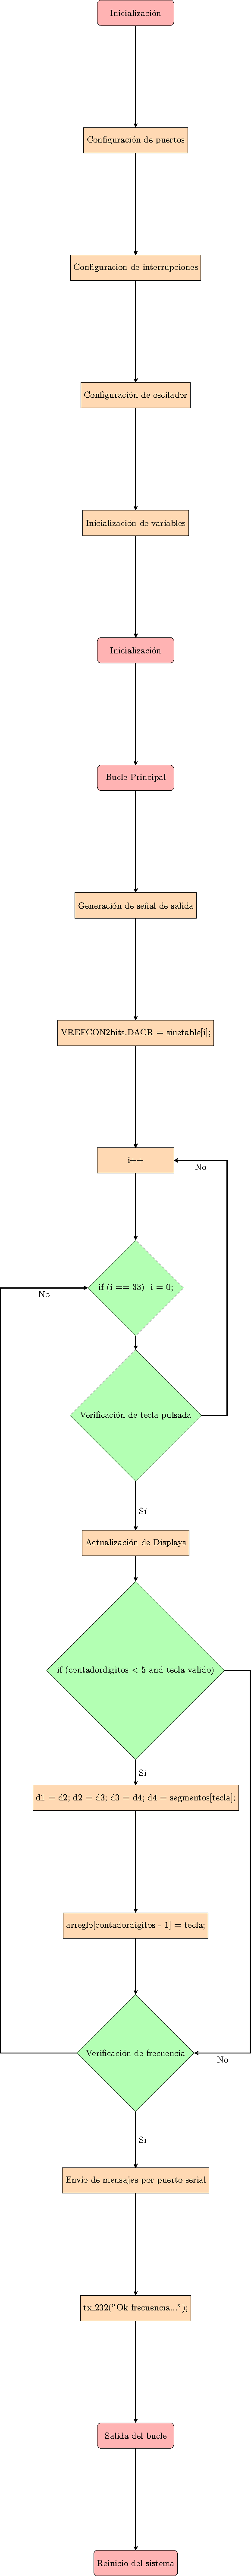
\includepdf{fmain.pdf}

\subsection{Interrupcion}
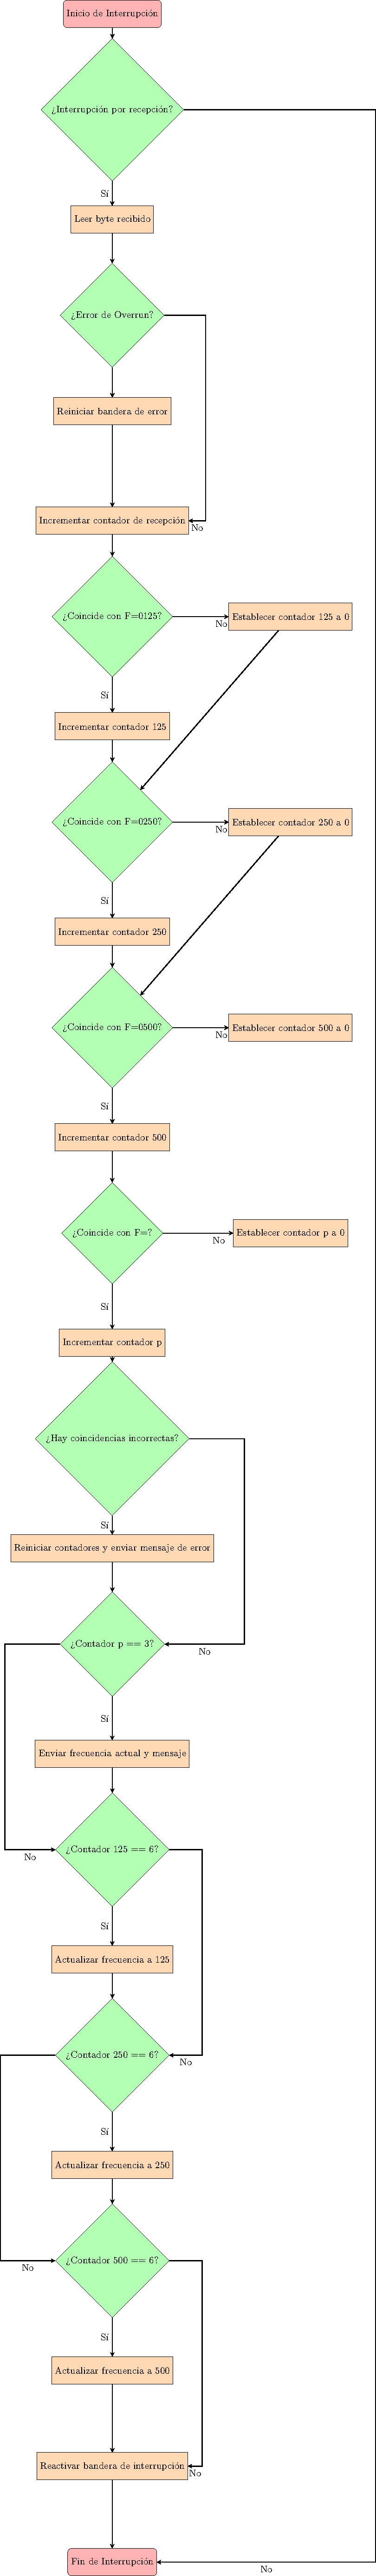
\includepdf{altainterrupcion.pdf}
\subsection{Comunicacion}
\begin{tikzpicture}[node distance=2.5cm]  

% Nodos para la función tx_232  
\node (start1) [startstop] {Inicio tx232};  
\node (checkLength) [decision, below of=start1] {¿longitud > 0?};  
\node (sendChar) [process, below of=checkLength, yshift=-0.5cm] {TXREG1 = *mens};  
\node (clearFlag) [process, below of=sendChar] {PIR1bits.TXIF = 0};  
\node (waitForSend) [process, below of=clearFlag] {Esperar a que TXIF = 1};  
\node (decrement) [process, below of=waitForSend] {longitud-- \\ mens++};  
\node (end1) [startstop, below of=decrement] {Fin tx232};  

% Nodos para la función Envia_cadena  
\node (start2) [startstop, right of=start1, xshift=4cm] {Inicio Enviacadena};  
\node (getLength) [process, below of=start2] {Cantidad = strlen(texto)};  
\node (setBuffer) [process, below of=getLength] {sprintf(buffer, texto)};  
\node (loopBuffer) [process, below of=setBuffer] {For (i=0; i<cantidad)};  
\node (bufferSend) [process, below of=loopBuffer] {TXREG1 = buffer[i]};  
\node (clearFlag2) [process, below of=bufferSend] {PIR1bits.TXIF = 0};  
\node (waitForSend2) [process, below of=clearFlag2] {Esperar a que TXIF = 1};  
\node (end2) [startstop, below of=waitForSend2] {Fin Enviacadena};  

% Nodos para la función Envia_frecuencia  
\node (start3) [startstop, right of=start2, xshift=4cm] {Inicio Enviafrecuencia};  
\node (initVars) [process, below of=start3] {cantdigitos = 0 \\ frecuencia1 = frecval};  
\node (whileLoop) [decision, below of=initVars] {¿frecuencia1 $>$ 0?};  
\node (countDigits) [process, below of=whileLoop, yshift=-0.5cm] {cantdigitos++ \\ frecuencia1 /= 10};  
\node (endWhile) [process, below of=countDigits] {sprintf(buffer, frecval)};  
\node (loopBuffer2) [process, below of=endWhile] {For (i=0; i<cantdigitos)};  
\node (bufferSend2) [process, below of=loopBuffer2] {TXREG1 = buffer[i]};  
\node (clearFlag3) [process, below of=bufferSend2] {PIR1bits.TXIF = 0};  
\node (waitForSend3) [process, below of=clearFlag3] {Esperar a que TXIF = 1};  
\node (end3) [startstop, below of=waitForSend3] {Fin Enviafrecuencia};  

% Conexiones para tx_232  
\draw [arrow] (start1) -- (checkLength);  
\draw [arrow] (checkLength) -- node[anchor=east]{Sí} (sendChar);  
\draw [arrow] (sendChar) -- (clearFlag);  
\draw [arrow] (clearFlag) -- (waitForSend);  
\draw [arrow] (waitForSend) -- (decrement);  
\draw [arrow] (decrement.east) --++ (1,0) --++(0,-2.5) -- node[anchor=south]{No} (end1.east);  
\draw [arrow] (checkLength.west) --++ (-1,0) --++(0,-13) -- node[anchor=south]{No} (end1.west);  

% Conexiones para Envia_cadena  
\draw [arrow] (start2) -- (getLength);  
\draw [arrow] (getLength) -- (setBuffer);  
\draw [arrow] (setBuffer) -- (loopBuffer);  
\draw [arrow] (loopBuffer) -- (bufferSend);  
\draw [arrow] (bufferSend) -- (clearFlag2);  
\draw [arrow] (clearFlag2) -- (waitForSend2);  
\draw [arrow] (waitForSend2.east) --++ (1,0) --++(0,-2.5) -- node[anchor=south]{No} (end2.east);  

% Conexiones para Envia_frecuencia  
\draw [arrow] (start3) -- (initVars);  
\draw [arrow] (initVars) -- (whileLoop);  
\draw [arrow] (whileLoop) -- node[anchor=east]{Sí} (countDigits);  
\draw [arrow] (countDigits) -- (whileLoop);  
\draw [arrow] (whileLoop.east) --++ (1.2,0) --++(0,-5.5) -- node[anchor=south]{No} (endWhile.east);  
\draw [arrow] (endWhile) -- (loopBuffer2);  
\draw [arrow] (loopBuffer2) -- (bufferSend2);  
\draw [arrow] (bufferSend2) -- (clearFlag3);  
\draw [arrow] (clearFlag3) -- (waitForSend3);  
\draw [arrow] (waitForSend3.east) --++ (1,0) --++(0,-2.5) -- node[anchor=south]{No} (end3.east);  

\end{tikzpicture} 
      \section{Conclusiones} 

En esta práctica, se implementó un convertidor digital-analógico (DAC) utilizando un muestreo controlado por un retardo en lugar de un temporizador. Esto permitió observar cómo se generaban diferentes frecuencias de salida a partir de valores digitales, lo que es fundamental en aplicaciones de procesamiento de señales. Al utilizar un retardo para el muestreo, se pudo observar cómo la frecuencia de salida variaba en función del tiempo de espera entre cada muestreo. Esto es crucial para entender cómo se puede manipular la señal de salida en un DAC. La implementación de la comunicación serial permitió cambiar dinámicamente la frecuencia de salida del DAC. Aprendí a utilizar el teclado para enviar comandos que modifican los parámetros de la señal, lo que demuestra la importancia de la interacción entre el usuario y el sistema. La comunicación serial es esencial en sistemas embebidos, ya que permite la configuración y el monitoreo en tiempo real de los dispositivos. Las imágenes del osciloscopio muestran diferentes formas de onda generadas por el DAC. A medida que se ajustaba la frecuencia, se podía observar cómo la forma de la señal cambiaba, lo que es indicativo de la calidad del muestreo y la resolución del DAC. Las variaciones en la frecuencia de muestreo también se reflejan en la forma de la señal, lo que resalta la importancia de un muestreo adecuado para obtener una representación precisa de la señal analógica. 

\begin{figure}[H]
      \centering
      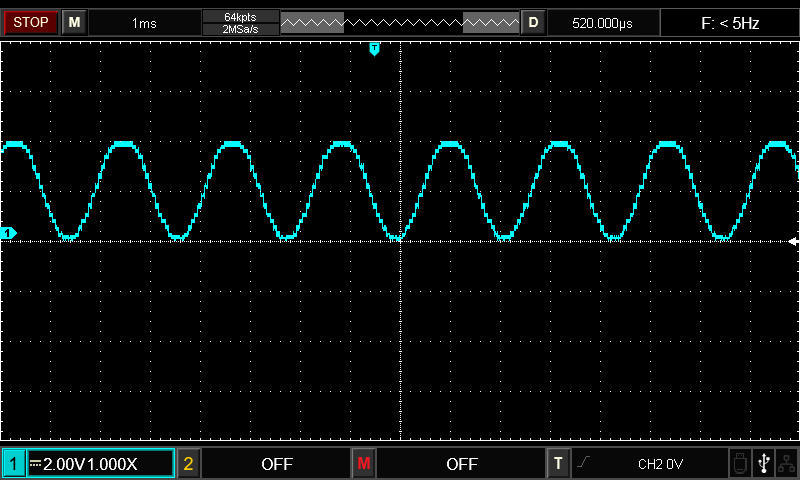
\includegraphics[width=0.5\textwidth]{images/500HZ}
      \captionof{figure}{Señal de $500\si{\Hz}$}
\end{figure}

\begin{figure}[H]
      \centering
      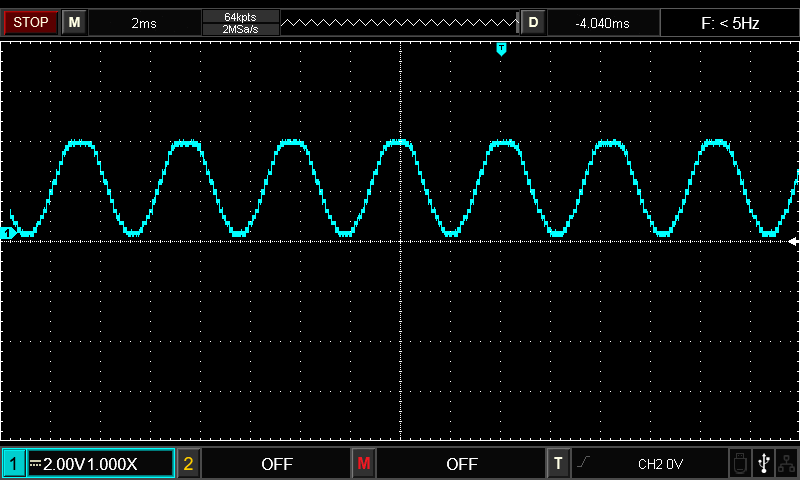
\includegraphics[width=0.5\textwidth]{images/250HZ}
      \captionof{figure}{Señal de $250\si{\Hz}$}
\end{figure}

\begin{figure}[H]
      \centering
      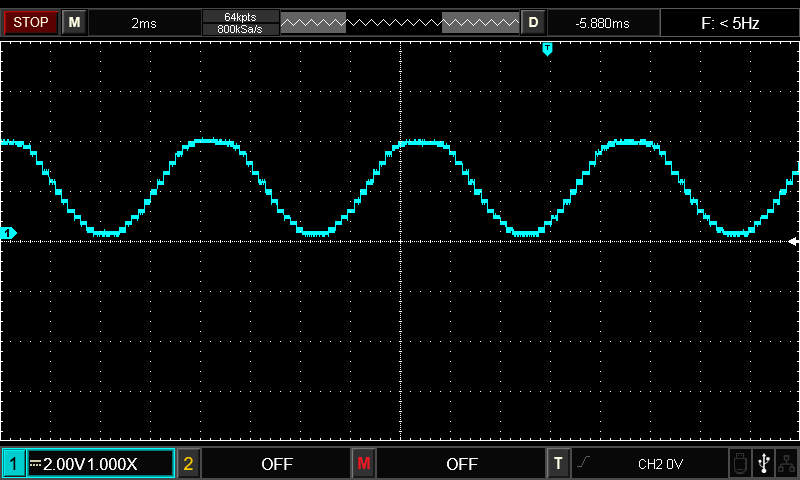
\includegraphics[width=0.5\textwidth]{images/125HZ}
      \captionof{figure}{Señal de $125\si{\Hz}$}
\end{figure}
\end{document}
